% XeLaTex
%\documentclass[review]{cvpr}
\documentclass[final]{cvpr}

\usepackage[UTF8]{ctex}

%\usepackage{cvpr}
\usepackage{times}
\usepackage{epsfig}
\usepackage{graphicx}
\usepackage{amsmath}
\usepackage{amssymb}
\usepackage{subfigure}
\usepackage{overpic}
\usepackage{color}
\usepackage{enumitem}
\setenumerate[1]{itemsep=0pt,partopsep=0pt,parsep=\parskip,topsep=5pt}
\setitemize[1]{itemsep=0pt,partopsep=0pt,parsep=\parskip,topsep=5pt}
\setdescription{itemsep=0pt,partopsep=0pt,parsep=\parskip,topsep=5pt}


\usepackage[pagebackref=true,breaklinks=true,colorlinks,bookmarks=false]{hyperref}


%\cvprfinalcopy % *** Uncomment this line for the final submission

\def\cvprPaperID{159} % *** Enter the CVPR Paper ID here
\def\confYear{CVPR 2020}
\def\httilde{\mbox{\tt\raisebox{-.5ex}{\symbol{126}}}}

\newcommand{\cmm}[1]{\textcolor[rgb]{0,0.6,0}{CMM: #1}}
\newcommand{\todo}[1]{{\textcolor{red}{\bf [#1]}}}
\newcommand{\alert}[1]{\textcolor[rgb]{.6,0,0}{#1}}

\newcommand{\IT}{IT\cite{98pami/Itti}}
\newcommand{\MZ}{MZ\cite{03ACMMM/Ma_Contrast-based}}
\newcommand{\GB}{GB\cite{conf/nips/HarelKP06}}
\newcommand{\SR}{SR\cite{07cvpr/hou_SpectralResidual}}
\newcommand{\FT}{FT\cite{09cvpr/Achanta_FTSaliency}}
\newcommand{\CA}{CA\cite{10cvpr/goferman_context}}
\newcommand{\LC}{LC\cite{06acmmm/ZhaiS_spatiotemporal}}
\newcommand{\AC}{AC\cite{08cvs/achanta_salient}}
\newcommand{\HC}{HC-maps }
\newcommand{\RC}{RC-maps }
\newcommand{\Lab}{$L^*a^*b^*$}
\newcommand{\mypara}[1]{\paragraph{#1.}}

\graphicspath{{figures/}}

% Pages are numbered in submission mode, and unnumbered in camera-ready
%\ifcvprfinal\pagestyle{empty}\fi
\setcounter{page}{1}

\begin{document}
% \begin{CJK*}{GBK}{song}

\renewcommand{\figref}[1]{图\ref{#1}}
\renewcommand{\tabref}[1]{表\ref{#1}}
\renewcommand{\equref}[1]{式\ref{#1}}
\renewcommand{\secref}[1]{第\ref{#1}节}
\def\abstract{\centerline{\large\bf 题目介绍} \vspace*{12pt} \it}

%%%%%%%%% TITLE

\title{机器学习第三次作业}

\author{朱一凡 \quad 计算机学院 \quad2120200467}

\maketitle
% \thispagestyle{empty}

%%%%%%%%% ABSTRACT
\begin{abstract}
    线性回归问题:数据文件 Dataset(5).csv 中包含 9 个训练样本点,组成\textcolor{blue}{训练样本集}。\par
    1)利用第四讲作业实现的线性回归最小二乘法得到训练样本集的最小二乘解,并且利用得到的线性回归模型生成5个测试样本,组成\textcolor{blue}{测试样本集},使用两种颜色绘出训练样本集和测试样本集中样本的散布图。假设噪声模型为$\mathcal{N}(0,5)$。\par
    2)编程实现岭回归算法,求解出训练样本集的岭回归模型,给出训练样本均方误差和测试样本均方误差。\par
    3)比较岭回归模型与线性回归模型(最小二乘解)的训练样本均方误差和测试样本均方误差,给出结论及理由。\par
    4)如果使用多项式回归模型来拟合训练样本集,应该选择多少阶的多项式?说明你给出此答案的理由\par
\end{abstract}




%%%%%%%%% BODY TEXT %%%%%%%%%%%%%%%%%%%%%%%%%%%%%%%%%%%%%%%%
\section{问题描述}
该问题依然是一个线性回归问题。需要根据给出的训练数据来进行测试数据的生成。同时使用最小二乘法线性回归和岭回归法线性回归来进行实验。并对比两者性能上的异同。主要是比较二者的训练均方误差和测试均方误差。另外考虑在使用多项式回归模型的时候需要选择几阶的多项式。
\section{基本思路}
对于数据生成阶段。需要观察所给出的训练数据在哪一个范围内,并生成对应范围内的数据。如果训练数据和测试数据之间的范围相差过大,也无法使用测试数据客观的来评价算法的性能。\par
对于最小二乘法回归模型,直接使用在第四讲实验中得到的结果即可。对于岭回归,可以在最小二乘法的基础上进行拓展。也比较容易实现。采取第四讲实验中的代码可以方便的计算出这两种算法的训练均方误差和测试均方误差并进行比较。因为没有特别说明,此处岭回归模型使用的也是线性回归模型。\par
在选取使用几阶多项式进行回归分析时,很重要的一点就是数据量的大小。可以通过分析所使用的训练数据的数量来确定最多使用几次的阶数。如果阶数过大将毫无意义。如果需要求出最优阶数,需要对能取到的阶数进行一个遍历。\par
\section{解题步骤}
接下来对问题的解决步骤进行更进一步的描述。主要分为处理流程,算法描述,算法实现几个步骤。
\subsection{处理流程}
首先,因为CSV中的数据量很少,所以可以直接将这些数据写到Python的代码里。但是如果有更多的数据时这一方法就不太方便。所以在此选择将其进行读取。绘图的相关代码使用上一次实验中所使用到的代码。\par
对于最小二乘法的实现,可以直接使用上一次实验中所使用到的代码。岭回归算法和最小二乘法的区别主要在于优化的目标和计算权值中所使用到的公式。所以使用最小二乘法的代码进行修改得到。在岭回归算法中,收缩因子的确定也是十分重要的。岭回归的收缩因子可以使用交叉验证的方法得到。在此我们首先确定最佳的收缩因子,随后利用该收缩因子的结果和最小二乘法的结果进行比较。同时为了得到更加一般的结果,重复实验100次,并将结果取平均进行比较。\par
对于多项式回归的阶数选择。首先将训练的图像绘制出来,大致的判断一下其形状。同时根据数据量进行一定的限制。如果最高的阶数过高,那么所得到的模型也是没有意义的。同时,可以使用程序编程实现来验证最后结果的正确性。因为题目中没有要求,这一部分的代码直接使用相关的机器学习算法库进行实现。
\subsection{算法描述}
首先进行数据的生成。观察给出的训练数据之后,在算法中使用均匀采样的方法在$[-2,2]$区间上采样5次得到$x$,随后使用公式$y = \hat{w_{1}}x+\hat{w_{0}} + \mathcal{N}(0,5)$。
来得到$y$的值。其中$ \hat{w_{1}}, \hat{w_{0}}$是最小二乘算法估计得到的参数。每一次的数据使用一个类函数来表达。绘制散点图可以使用Python中的matplotlib库
进行实现。由于随机数的生成具有不确定性,所以进行多次生成以确保算法的有效性。\par
在得到训练数据和测试数据之后,可以进行回归算法的实现。对于最小二乘法来说,在处理线性回归时,可以使用以下的公式进行计算
\begin{equation}
    \hat{w} = (X^TX)^{-1}X^Ty
\end{equation}
均方误差可以使用以下公式进行计算
\begin{equation}
    MSE = \sum_{i=0}^{n}{(y-\hat{y})^2}
\end{equation}
对于岭回归算法来说,在处理线性回归时,可以使用以下的公式进行计算
\begin{equation}
    \hat{w} = (X^TX+\lambda I)^{-1}X^Ty
\end{equation}
均方误差可以使用以下公式进行计算
\begin{equation}
    MSE = \sum_{i=0}^{n}{(y-\hat{y})^2}
\end{equation}

\subsection{算法实现(Python语言源代码)}
算法的实现结果如附件中的代码所示。使用Python语言实现,主要使用了numpy,matplotlib,pytorch算法库。其中最小二乘法和岭回归算法均使用自己编写的程序实现。在确定最优的多项式回归阶数时,使用已有的算法库进行实现。
\section{结果与分析}
\subsection{实验内容与步骤}
首先通过给出的数据计算出最小二乘线性模型,随后使用得到的模型参数生成测试样本。然后使用岭回归算法进行回归,并在每一次确定出最优的$\lambda$参数。这一参数可以使用交叉验证的的方法得到。然后将最小二乘法的结果和岭回归法的结果进行比较分析。最后通过给定数据的形状分布和数量来综合确定使用多项式回归时应当使用的系数。
\subsection{实验结果}
给定的训练数据的数据分布情况如图\ref{data}(a)所示。经过计算得到的最小二乘法线性模型结果为:
最小二乘法:$y = 1.97666667x-1.66533454*10^{-16}$, $MSE = 7.94$\par
根据上述公式生成5个测试样本,训练样本和测试样本的分布如图\ref{data}(b)所示。
\begin{figure}[htbp]
    \centering
    \subfigure[训练数据分布]{
    \begin{minipage}[t]{0.5\linewidth}
    \centering
    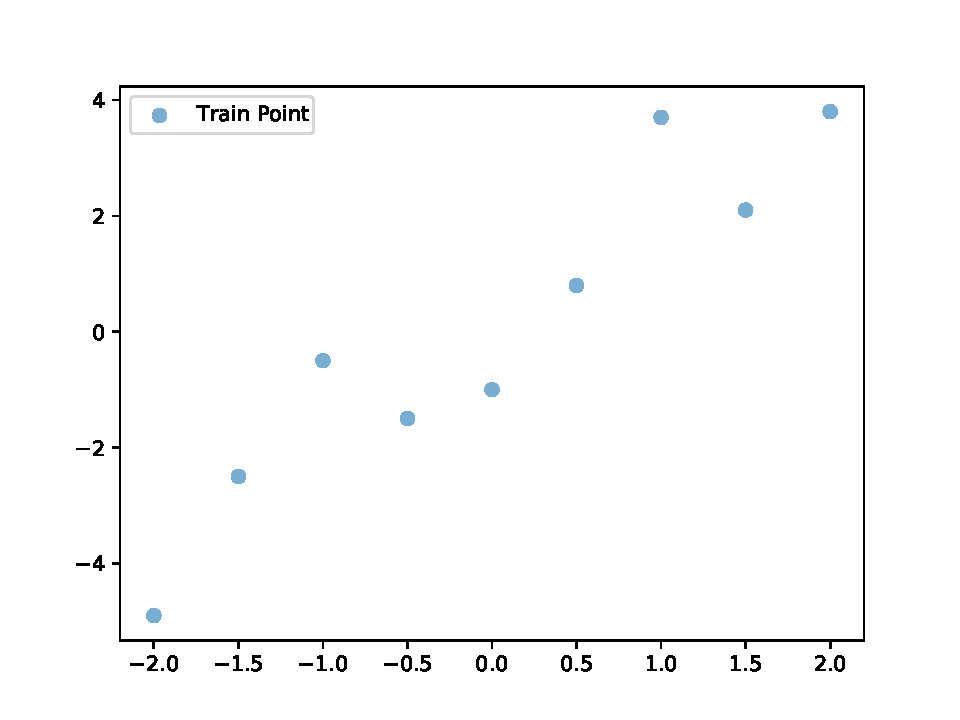
\includegraphics[width=3.5in]{figures/train_point.pdf}
    \end{minipage}%
    }%
    \subfigure[训练数据和生成的测试数据分布]{
    \begin{minipage}[t]{0.5\linewidth}
    \centering
    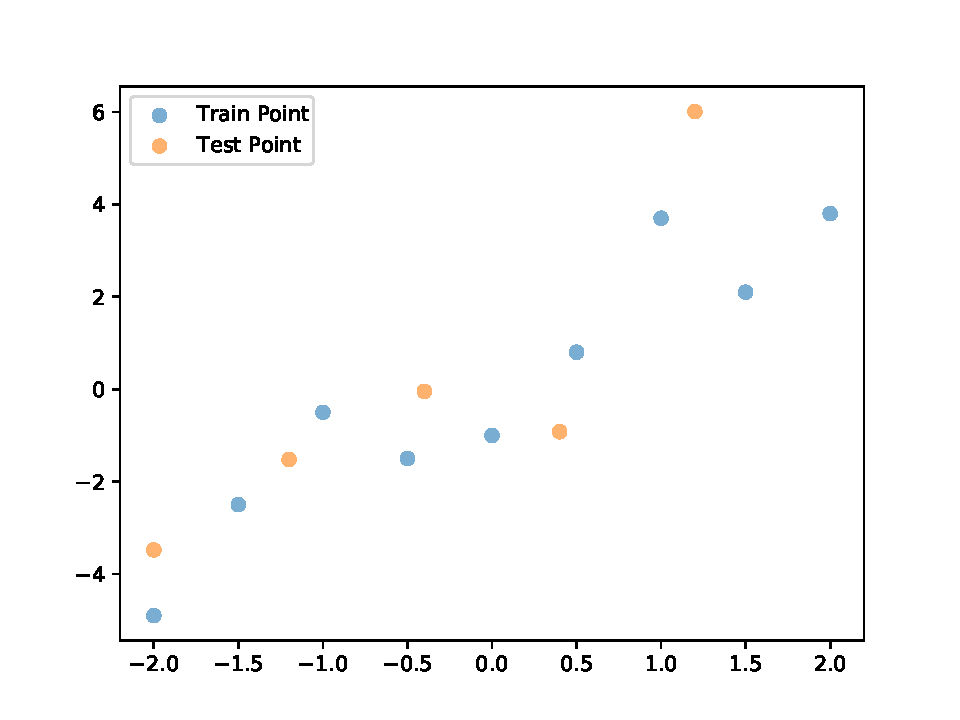
\includegraphics[width=3.5in]{figures/train_test_point.pdf}
    %\caption{fig2}
    \end{minipage}%
    }%   
\caption{数据的分布}
\label{data}               
\end{figure}
通过不断的改变收缩因子进行计算,可以得到训练误差,测试误差随着收缩因子的变化曲线。图\ref{lambda}(a)中,收缩因子的变化范围为[-10,20]可以看到随着收缩因子的不断变化,最终的结果逐渐从欠拟合变化到了过拟合。同时计算得出比较合适的$\lambda$为$-6$。同时,在实验中发现了一个十分有意思的情况,当收缩因子为$-15$的时候,训练误差和测试误差都发生了爆炸。这一问题的具体原因还未能解决。\par
\begin{figure}[htbp]
    \centering
    \subfigure[收缩因子范围为-10到20]{
    \begin{minipage}[t]{0.5\linewidth}
    \centering
    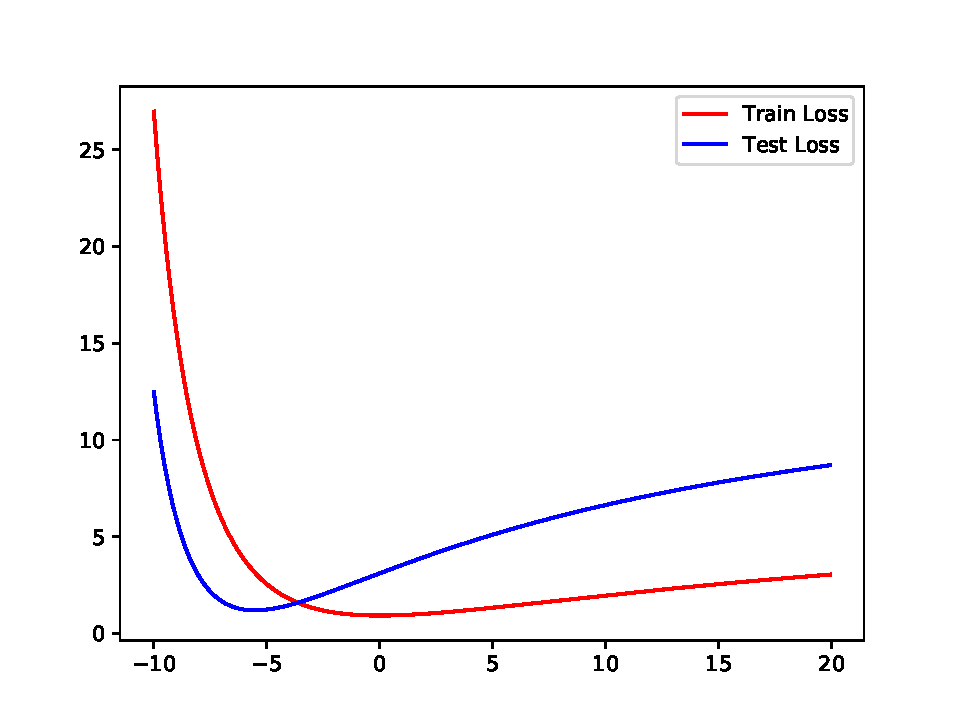
\includegraphics[width=3.5in]{figures/Ridge_lambda.pdf}
    \end{minipage}%
    }%
    \subfigure[收缩因子范围为-20到20]{
    \begin{minipage}[t]{0.5\linewidth}
    \centering
    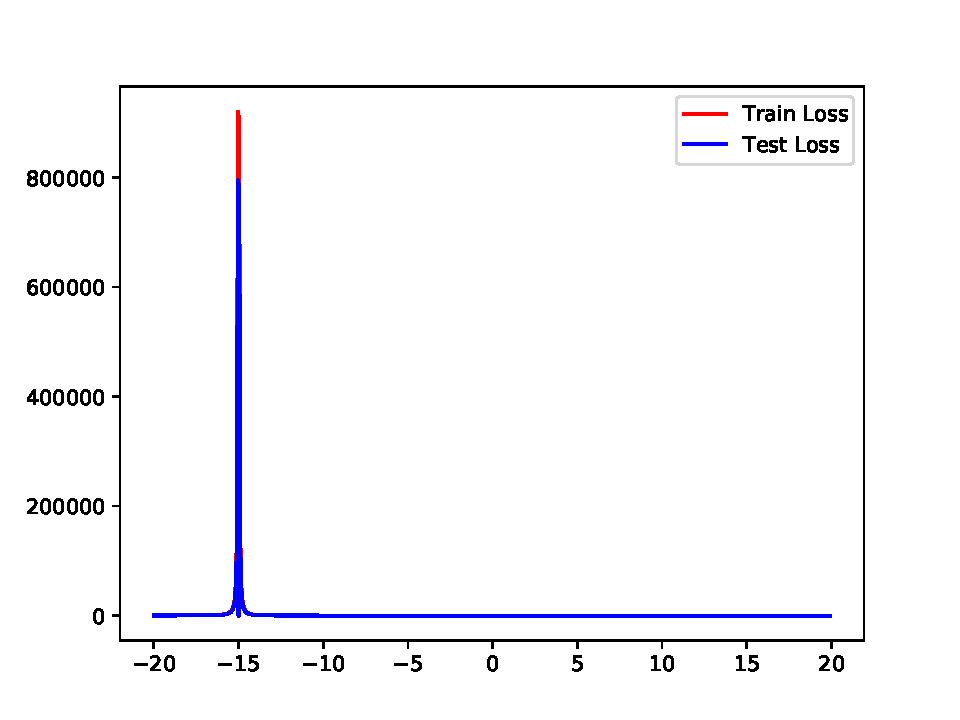
\includegraphics[width=3.5in]{figures/Ridge_lambda2.pdf}
    %\caption{fig2}
    \end{minipage}%
    }%
\caption{收缩因子变化的影响}
\label{lambda}       
\end{figure}
最终结果:\par
最小二乘法:$y = 1.97666667x-1.66533454*10^{-16}$, $Train\_MSE = 0.9257592592592593$, $Test\_MSE = 3.524157405398151$\par
岭回归:$y = 3.29444444x$, $Train\_MSE = 3.8199897119341557$, $Test\_MSE = 2.5635166310052195 $ \par
算法的结果图如图\ref{compare}所示。可以看到在测试的时候岭回归的结果会更好一些。\par
\begin{figure}[htbp]
    \centering
    \subfigure[最小二乘法]{
    \begin{minipage}[t]{0.5\linewidth}
    \centering
    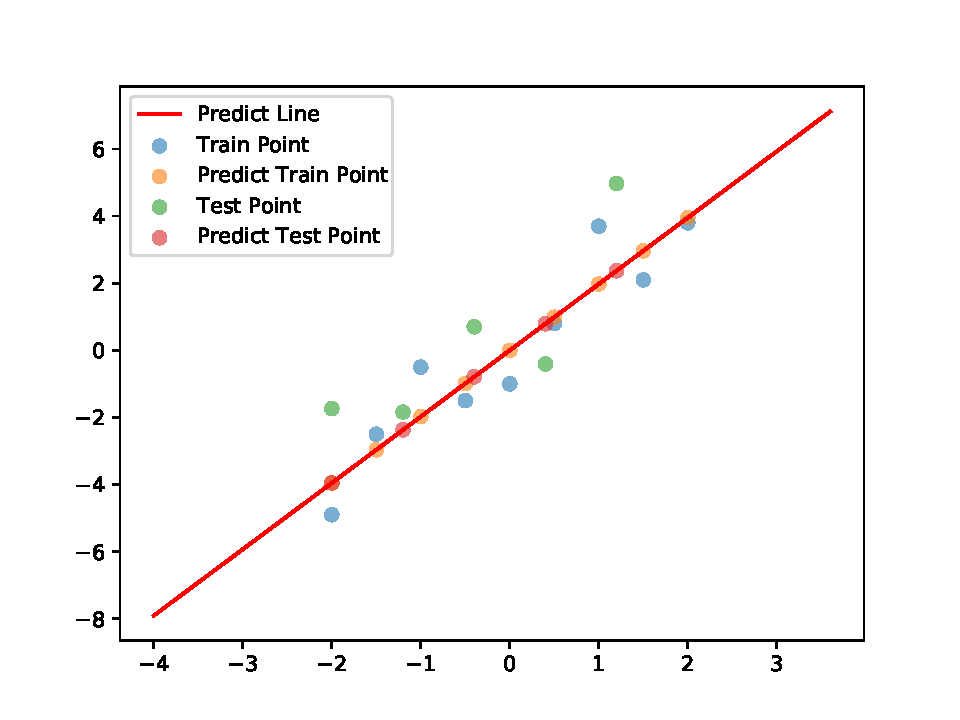
\includegraphics[width=3.5in]{figures/LeastSquares.pdf}
    \end{minipage}%
    }%
    \subfigure[岭回归法($\lambda=-6$)]{
    \begin{minipage}[t]{0.5\linewidth}
    \centering
    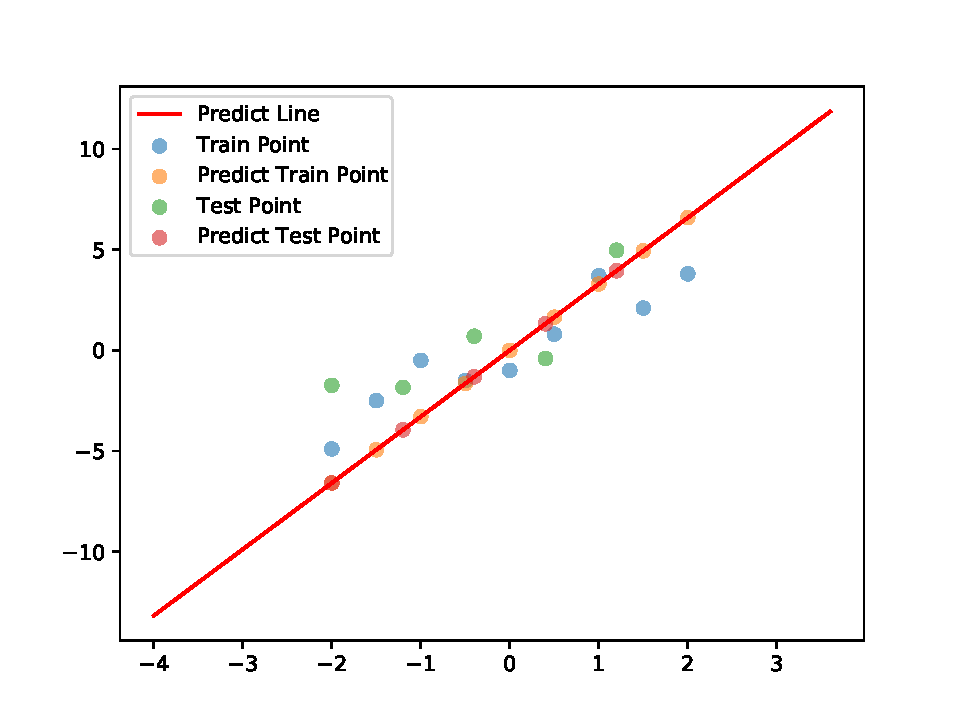
\includegraphics[width=3.5in]{figures/Ridge.pdf}
    %\caption{fig2}
    \end{minipage}%
    }%   
\caption{算法结果对比}
\label{compare}               
\end{figure}

观察图\ref{poly}中的数据分布,大致可以观察出使用$5$次曲线来进行拟合会更好。因为图像一共有四个极值点,所以用五次多项式来拟合效果会更好一些。使用多项式拟合算法库进行测试之后的loss变化图像如图所示。可以看到,阶数为9的时候效果最好,但是我认为这是不合理的,这是因为出现了过拟合现象。
\begin{figure}[]
    \centering
    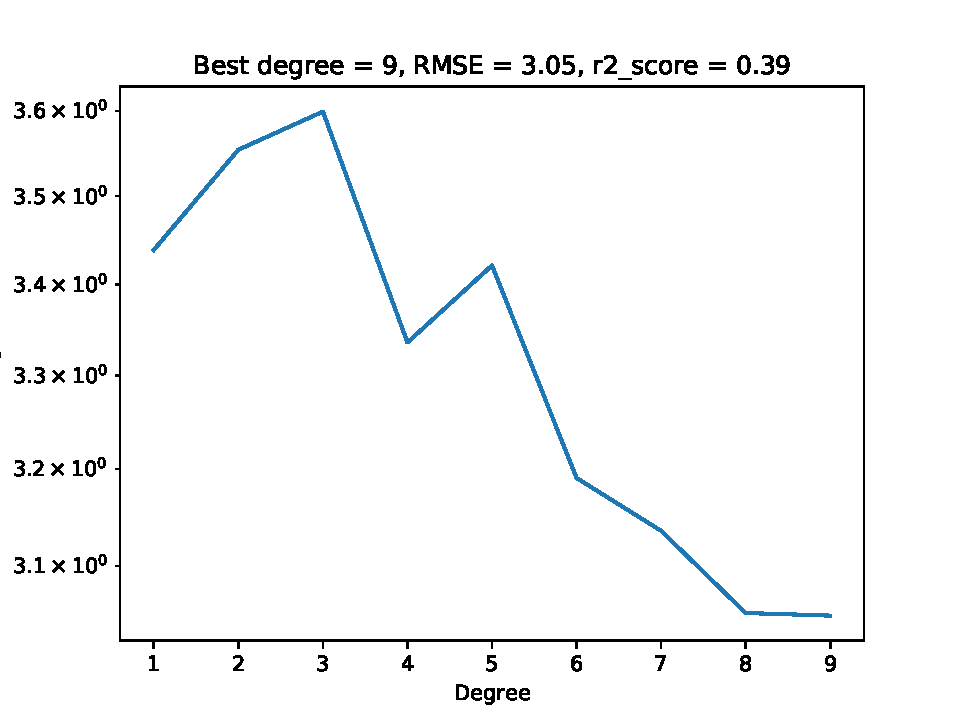
\includegraphics{figures/poly.pdf}
\caption{多项式阶数选取}
\label{poly}               
\end{figure}
\subsubsection{结果分析}
首先是最小二乘法和岭回归结果的分析。可以看到最小二乘法的训练均方误差结果要远远好于岭回归的方法。但是在测试均方误差的表现上,岭回归要比最小二乘回归的结果更好。这是因为岭回归不仅考虑了训练时的训练误差,还考虑到了模型参数对于算法模型的影响。\par
线性回归模型的基本假设满足时,用最小二乘法得到的回归系数估计量是无偏的且具有最小方差,即使在高度多重相关的情况下,最小二乘法的回归系数估计量依然是线性无偏的,且具有最小的方差,也就是说多重共线性并不影响最小二乘估计量的无偏性和最小方差性。因此在所有的线性无偏估计中,最小二乘估计仍然具有较小的方差,但这并不意味着最小二乘的估计量的方差一定是最小的,因为虽然它在所有线性无偏估计量中方差较小,但是该值确不一定是最好的。岭回归就是一种放弃无偏估计性要求的方法。\par
在确定多项式拟合的最优阶次时,已经预料最终效果最好的阶数应该是9.因为所给出的数据量太少了,很容易就会出现这种过拟合的现象。因为使用的是封装好的算法,所以并没有对其中细节进行更进一步的改进。但是正确的阶数一定要比8小,因为九个数据最高能确定的也就是8次了。
%%%%%%%%%%%%%%%%%%%%%%%%%%%%%%%%%%%%%%%%%%%%%%%%%
\section{总结}\label{sec:Conclusion}
通过这一次的实验我明白到了正则化对于机器学习算法的重要意义。而且熟悉了另外的回归模型。岭回归模型是一种优秀的回归模型,但是还是要确定一个恰当的参数。在实验中的观察说明可能参数选取不恰当会产生很差的模型拟合效果。\par
在多项式拟合问题上也是如此,很难确定一个合适的阶数,需要人工仔细的分析和经验的加成。算法设计的复杂性还是十分明显的。




% \end{CJK*}
\end{document}
